% GenAU dialogue examples (Fig. A6, \label{fig:text}).
% Drawn at exactly the CVPR \textwidth (17.4625cm) so that
% 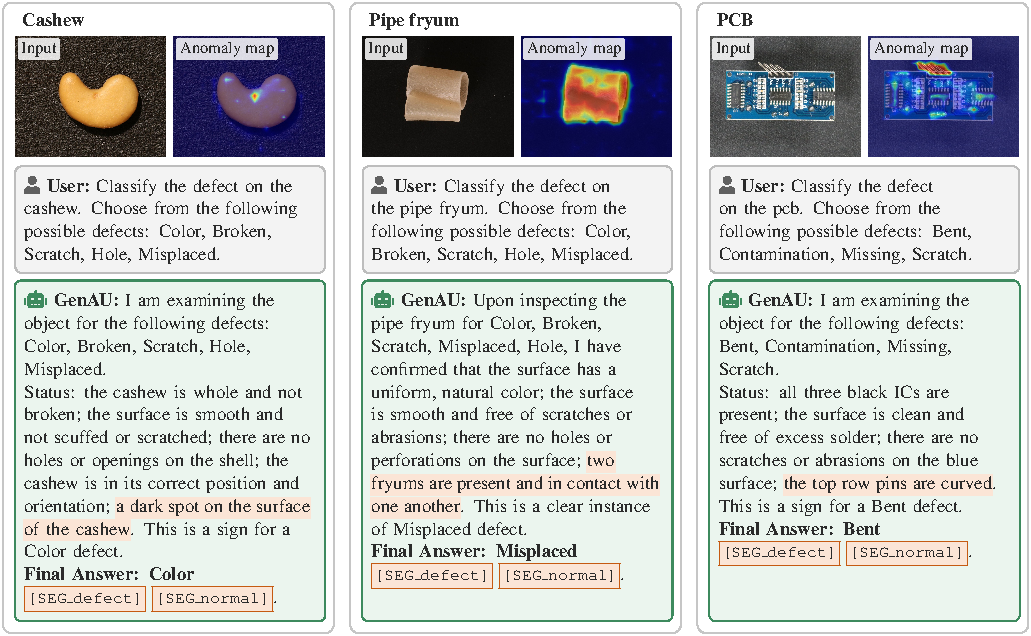
\includegraphics[width=\textwidth]{imgs/GenAU_Dialogue.pdf} places it at 1:1:
% Times 9pt text, same palette and [SEG] chips as Fig. 2 (imgs/GenAU_Arch.tex).
% Prompts and responses are the model transcripts of the earlier imgs/text.pdf,
% verbatim except the model name (GenAU) and the [SEG] token spelling of the paper.
% Build (from this directory):  pdflatex GenAU_Dialogue.tex  ->  GenAU_Dialogue.pdf
\documentclass[10pt]{standalone}
\usepackage{times}
\usepackage{graphicx}
\usepackage{fontawesome5}
\usepackage{soul}
\usepackage{tikz}
\usetikzlibrary{calc,backgrounds}

\definecolor{ink}{HTML}{2B2B2B}
\definecolor{txtS}{HTML}{3D8A5E}\definecolor{txtF}{HTML}{E2F1E7}
\definecolor{segS}{HTML}{C55A11}\definecolor{segF}{HTML}{FBE5D6}
\definecolor{datS}{HTML}{A0A0A0}\definecolor{datF}{HTML}{F3F3F3}

\sethlcolor{segF}  % \hl{...}: the observation the answer rests on
\newcommand{\seg}[1]{{\setlength{\fboxsep}{1pt}\setlength{\fboxrule}{0.4pt}%
  \fcolorbox{segS}{segF}{\footnotesize\ttfamily\strut #1}}}
\newcommand{\user}{\textcolor{datS!60!black}{\faUser}~\textbf{User:}~}
\newcommand{\genau}{\textcolor{txtS}{\faRobot}~\textbf{GenAU:}~}
\newcommand{\final}[1]{\textbf{Final Answer: #1} \seg{[SEG\_defect]}~\seg{[SEG\_normal]}.}

% one card: #1 index, #2 left x, #3 title, #4 image stem, #5 prompt, #6 response
\newcommand{\card}[6]{%
  \node[anchor=base west, font=\small\bfseries] at (#2+0.2,-0.4) {#3};
  \node[inner sep=0, anchor=north west] (in#1) at (#2+0.2,-0.55)
    {\includegraphics[width=2.56cm]{a6_#4_input.jpg}};
  \node[inner sep=0, anchor=north west] (mp#1) at (#2+2.88,-0.55)
    {\includegraphics[width=2.56cm]{a6_#4_map.jpg}};
  \node[tag] at ($(in#1.north west)+(0.05,-0.05)$) {Input};
  \node[tag] at ($(mp#1.north west)+(0.05,-0.05)$) {Anomaly map};
  \node[bubble, draw=datS!70, fill=datF, minimum height=\userh] (u#1)
    at ($(in#1.south west)+(0,-0.15)$) {\user #5};
  \node[bubble] (g#1) at ($(u#1.south west)+(0,-0.12)$) {\genau #6};
}

\begin{document}
\begin{tikzpicture}[
  x=1cm, y=1cm, font=\small, text=ink,
  tag/.style={anchor=north west, fill=white, fill opacity=0.85, text opacity=1,
              rounded corners=1pt, inner sep=1.5pt, font=\footnotesize},
  bubble/.style={anchor=north west, text width=4.94cm, align=left, inner sep=0.15cm,
                 rounded corners=3pt, line width=0.5pt,
                 execute at begin node={\hyphenpenalty=10000\exhyphenpenalty=10000}},
]
\def\userh{0cm}

\card{1}{0.05}{Cashew}{cashew}
  {Classify the defect on the cashew. Choose from the following possible defects:
   Color, Broken, Scratch, Hole, Misplaced.}
  {I am examining the object for the following defects: Color, Broken, Scratch, Hole,
   Misplaced.\\ Status: the cashew is whole and not broken; the surface is smooth and not
   scuffed or scratched; there are no holes or openings on the shell; the cashew is in its
   correct position and orientation; \hl{a dark spot on the surface of the cashew}. This is
   a sign for a Color defect.\\ \final{Color}}

\card{2}{5.93}{Pipe fryum}{fryum}
  {Classify the defect on the pipe fryum. Choose from the following possible defects:
   Color, Broken, Scratch, Hole, Misplaced.}
  {Upon inspecting the pipe fryum for Color, Broken, Scratch, Misplaced, Hole, I have
   confirmed that the surface has a uniform, natural color; the surface is smooth and free
   of scratches or abrasions; there are no holes or perforations on the surface; \hl{two
   fryums are present and in contact with one another}. This is a clear instance of
   Misplaced defect.\\ \final{Misplaced}}

\card{3}{11.81}{PCB}{pcb}
  {Classify the defect on the pcb. Choose from the following possible defects: Bent,
   Contamination, Missing, Scratch.}
  {I am examining the object for the following defects: Bent, Contamination, Missing,
   Scratch.\\ Status: all three black ICs are present; the surface is clean and free of
   excess solder; there are no scratches or abrasions on the blue surface; \hl{the top row
   pins are curved}. This is a sign for a Bent defect.\\ \final{Bent}}

% common bottom: the three answer bubbles and cards end on one line
\path let \p1=(g1.south), \p2=(g2.south), \p3=(g3.south) in
  \pgfextra{\pgfmathsetmacro{\yb}{min(\y1,\y2,\y3)}\xdef\yb{\yb pt}};
\begin{scope}[on background layer]
  \foreach \k/\x in {1/0.05, 2/5.93, 3/11.81}{
    \draw[datS!60, line width=0.5pt, rounded corners=4pt, fill=white]
      (\x,0) rectangle ($(\x+5.6,0)+(0,\yb)+(0,-0.2)$);
    \draw[txtS, line width=0.5pt, rounded corners=3pt, fill=txtF!70]
      (g\k.north west) rectangle (g\k.east |- 0,\yb);
  }
\end{scope}
\path (0,0.05) -- (17.4625,0.05);
\path (0,0) ++(0,\yb) ++(0,-0.25);
\end{tikzpicture}
\end{document}
